
%==========================================================================

\begin{frame}[fragile]

  {\Huge Organizational}

  \vspace{15pt}

  \textbf{Content:}
  \begin{itemize}
    \item Kokkos User Group @ HPSF Conference '26 (US)
    \item Mailing Lists
  \end{itemize}

\end{frame}

%==========================================================================

\begin{frame}[fragile]{Kokkos User Group 2026 (USA)}
  \begin{center}
    \textbf{Kokkos User Group @ HPSF Conference, USA}
  \end{center}

  \begin{itemize}
    \item \textit{When:} March 16th-20th 2026
    \item \textit{Where:} Chicago, IL, USA
    \item \textit{What:} 2\sfrac{1}{2}-days HPSF plenary + 2\sfrac{1}{2}-days Project meetings
    \item \textit{KUG-Content:} Focused on user experiences
    \begin{itemize}
	  \item Bring together Kokkos developers, library maintainers, and application teams.
      \item Share updates on performance portability work across the Kokkos ecosystem.
      \item Discuss topics including GPU performance tuning, interoperability (especially with Fortran), memory management, and distributed execution.
    \end{itemize}
  \end{itemize}

  \begin{center}
    \textit{Field Report for the Kokkos User Group Meeting 2026}\\
    \url{https://kokkos.org/blog/2026-03-KUG-report/}
  \end{center}
  
  \begin{textblock}{3}(12.5,3.5)
    
\includegraphics[width=0.9\textwidth]{5_1/Conference.png}
  \end{textblock}
\end{frame}

%==========================================================================

\begin{frame}[fragile]{Citing Kokkos - Help us track the impact of Kokkos}

\begin{itemize}
\item Ensure reproducibility
  \begin{itemize}
  \item Version-specific citations for Core and Kernels since 5.0
  \item Format: \emph{Kokkos Core v5.0.2, DOI: 10.5281/zenodo.18408291}
  \item See \href{https://kokkos.org/about/releases/}{release page} to find the specific DOI for the version you used
  \end{itemize}
\item In addition to that, please also cite relevant papers describing the component of the Ecosystem you used
\end{itemize}

Visit \url{https://kokkos.org/citing-kokkos/}

\end{frame}

%==========================================================================

\begin{frame}[fragile]{Tea-Time Webinar Series}

\begin{columns}
\column{0.5\textwidth}
\begin{itemize}
\item On the 3rd Wednesday of the month at 4 PM Paris time (usually 10 AM Eastern, 8 AM Mountain, 11 PM Tokyo time)
\item Find the playlist on \href{https://youtube.com/playlist?list=PLRKq_yxxHw2-Dkc4rEo8s-b3uaxJfuavA&si=BTBwI65FpP7B08uw}{HPSF YouTube channel}
\item Reach out if you would like to get invited to speak
\end{itemize}

\column{0.5\textwidth}
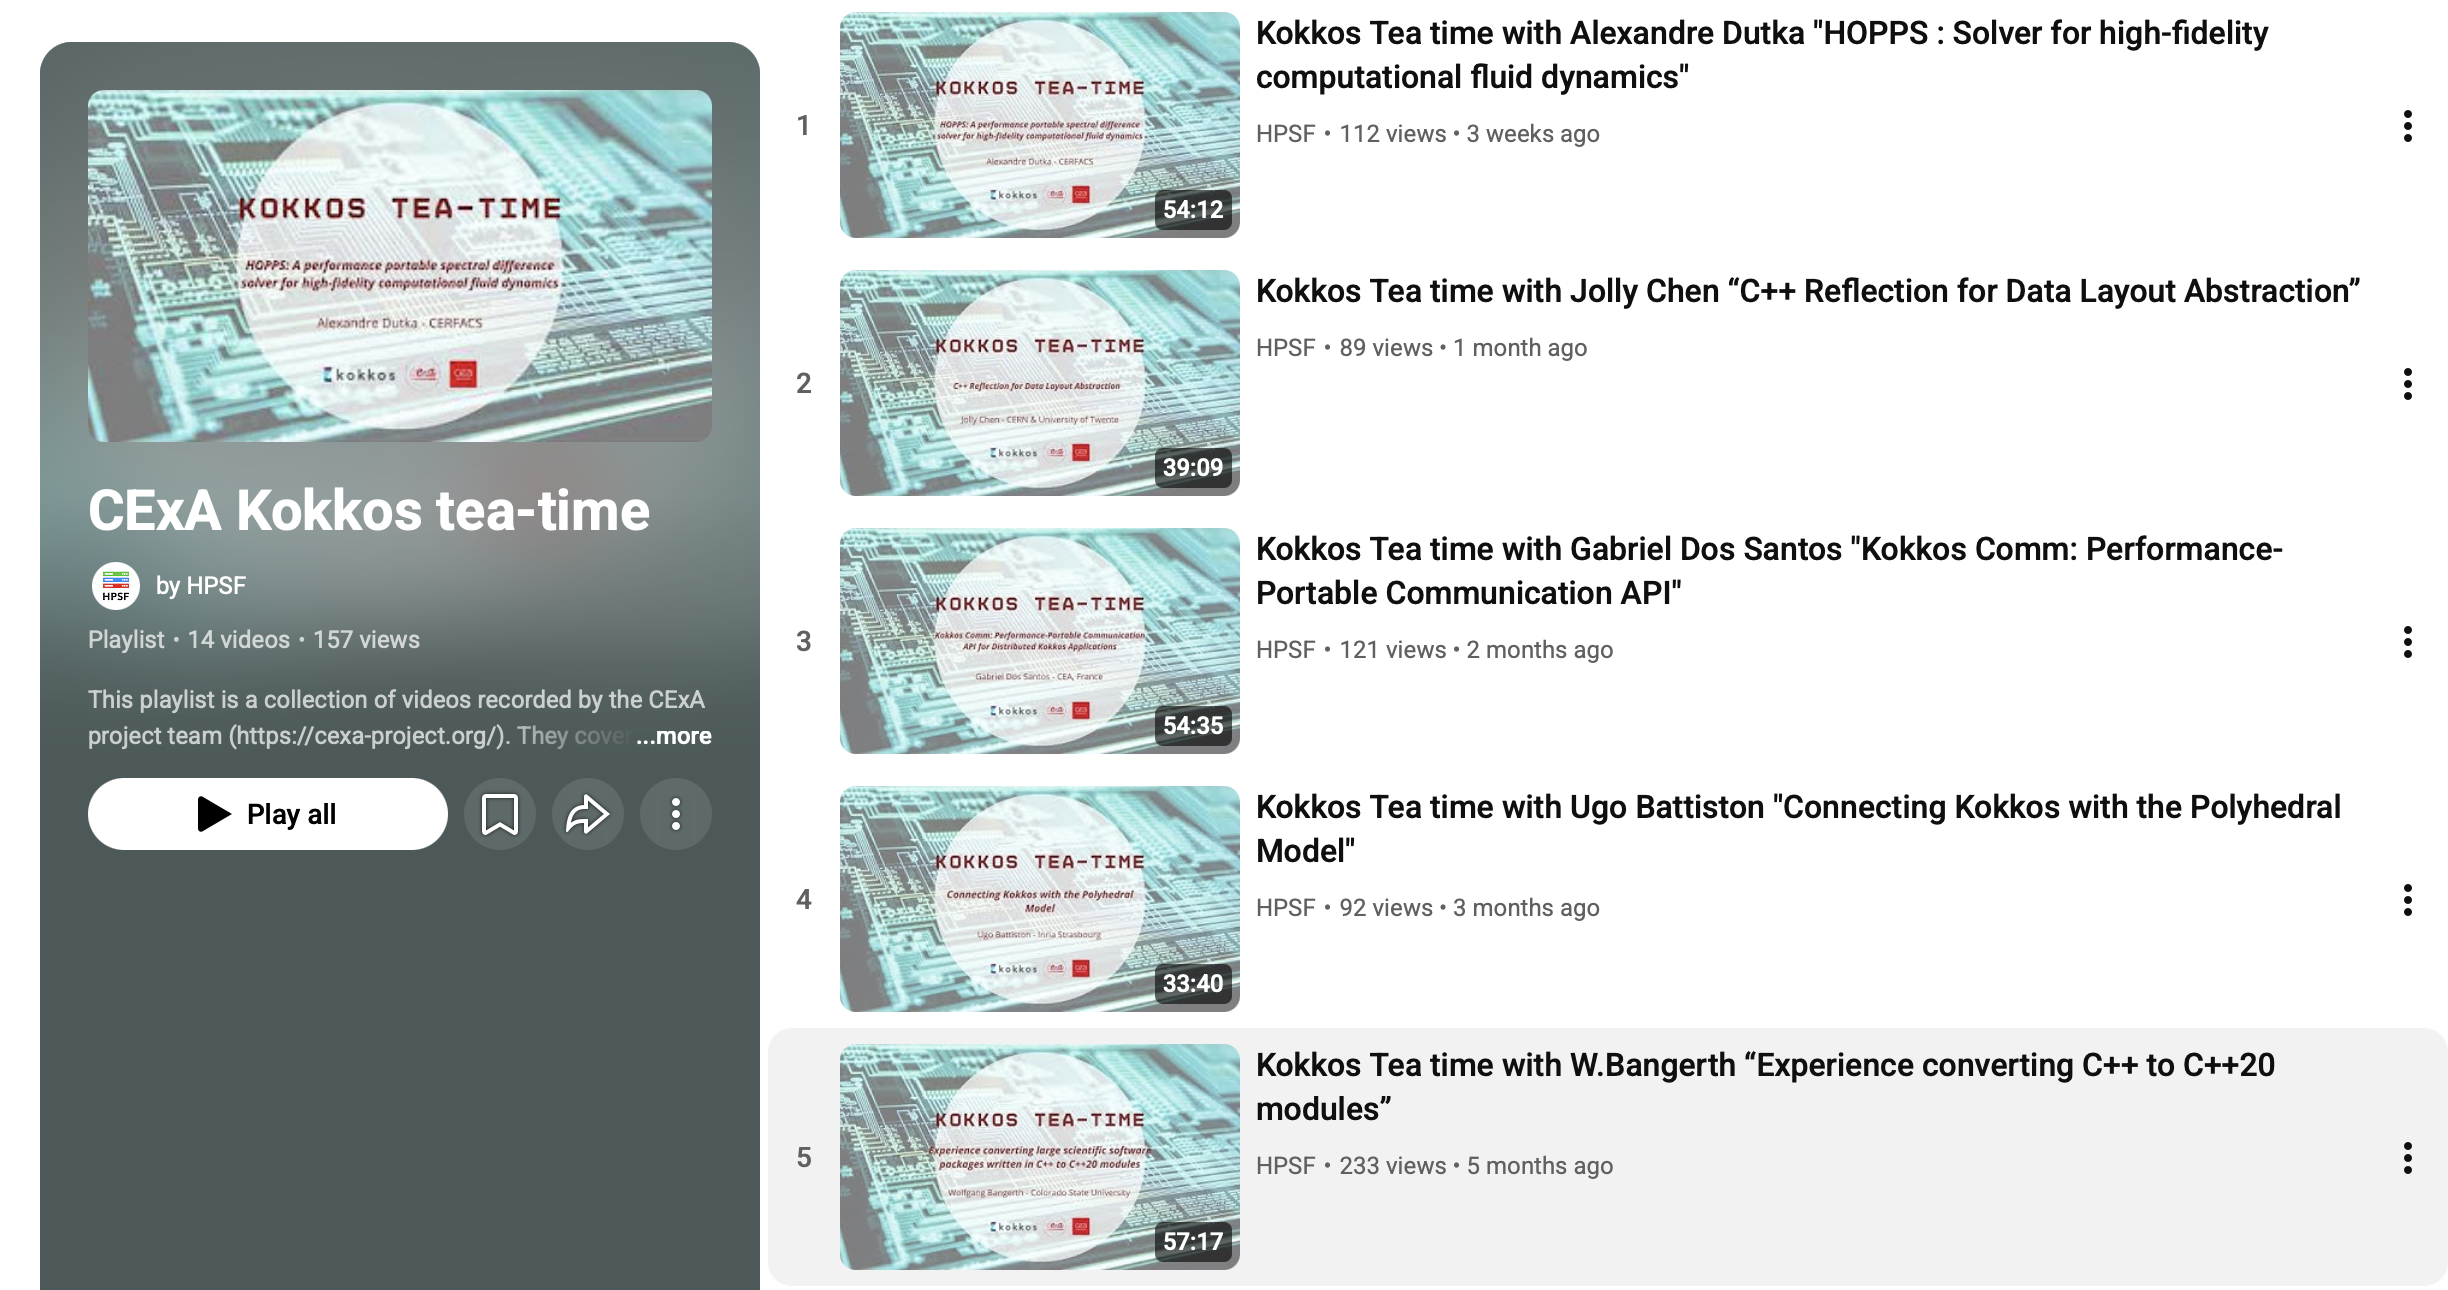
\includegraphics[width=\linewidth]{5_1/kokkos-tea-time-playlist.png}
\end{columns}

\begin{block}{Next session scheduled for tomorrow}
\emph{Parthenon – a performance portable block-structured adaptive mesh refinement framework}
by Philipp Grete
\end{block}

Visit \url{https://kokkos.org/community/tea-time/}

\end{frame}

%==========================================================================

\begin{frame}[fragile]{Other news}

\medskip

\begin{center}
  \textbf{Mailing Lists}\hspace{5em}~\\
  Sign up for the Kokkos mailing list to stay up-to-date\hspace{5em}~\\
  with the latest Kokkos news.\hspace{5em}~\\
  \url{https://kokkos.org/community/mailing-lists/}\hspace{5em}~
\end{center}
\medskip
\begin{textblock}{2}(12.5,9.75)
  
\includegraphics[width=\textwidth]{5_1/MLs.png}
\end{textblock}

\end{frame}

%==========================================================================

% Examples

% note: always keep the [fragile] for your frames!

%\begin{frame}[fragile]{Example list}
%  \begin{itemize}
%      \item Item 1
%      \item Item 2 with some \texttt{code}
%      \begin{itemize}
%        \item Sub-item 2.1
%        \item Sub-item 2.2
%      \end{itemize}
%  \end{itemize}
%\end{frame}

%\begin{frame}[fragile]{Example code}
%    \begin{code}[keywords={std}]
%        #include <iostream>
%
%        int main() {
%            std::cout << "hello world\n";
%        }
%    \end{code}
%\end{frame}

%\begin{frame}[fragile]{Example table}
%    \begin{center}
%        \begin{tabular}{l|l}
%            a & b \\\hline
%            c & d
%        \end{tabular}
%    \end{center}
%\end{frame}

%==========================================================================

